\chapter{Finding, Filtering, and Managing Information}
\begin{quote}
  In an information-rich world, the wealth of information means a dearth of something else: a scarcity of whatever it is that information consumes. What information consumes is rather obvious: it consumes the attention of its recipients. Hence a wealth of information creates a poverty of attention and a need to allocate that attention efficiently among the overabundance of information sources that might consume it.
\attrib{Herbert Simon \cite{simon1971designing}}
\end{quote}

\newthought{In a classroom evironment,} at almost every level, students are given the sources that they're expected to gather information from. They're assigned a textbook or papers to read. Students are never in a position where they're forced to evaluate the quality of several textbooks before deciding which to sink time into.

It's maybe no suprise, then, that most people develop, instead of hearty brain matter, a brothy-soup in their heads that comes \textit{this close} to spilling out whenever they sneeze.

How to do research is a skill that's rarely taught, and never taught
well. That's where this text comes in. I'm going to teach you how to realize
that you have a research problem and what to do about. I'll reveal the tricks
and techniques that I've picked up through years as an infovore.

There are, broadly speaking, four steps to information gathering.

\begin{enumerate}
  \item Realizing that information would improve of illuminate the situation
  \item Gathering all possibly relevant information and sources
  \item Filtering out the irrelevant bits
  \item Processing the information and recording what's relevant
\end{enumerate}

\section{Recognizing an opportunity}

\newthought{Today, the world is awash} in information, a constant deluge of the
stuff. A bitter, acrid sea that scours the world's digital stage and leaves a
trail of blog comments in its wake.

Supposing that tomorrow you were transported to some platonic
library\marginnote{``I have always imagined that Paradise will be a kind of
  library.'' Jorge Luis Borges}, staffed
by stern but fair angels who mute mp3 players with a wiggle of the wing, where
you never needed to sleep or eat, such that you could read constantly, it would
still take you about 62,000 years to read all the books that currently
exist. Or, about the time spanned from the first human crunching Australia's
long grass
beneath his feet until
now.  \marginnote{``Basically what Shannon said is that we define information as the opposite of uncertainty. If you have uncertainty, you don't have information. And once you receive information, uncertainty is being resolved.'' Martin Hilbert}

If that is not tantalizing enough, consider the case of Shaun Winterton. One May day in 2011, he discovered a new species of green lacewing, a dragonfly-esque insect.

Where did he find it, you might wonder -- braving ornery Amazonian black Caiman
or hunched over with yellow fever, praying for compassionate, generous death to just take him, maybe? But no. He discovered it not from the
eerie glow of a crocodile's eyes at night, but from the eerie glow of the the
photo-sharing website Flickr on his monitor. A new species! Advancing human
knowledge! From his couch.\cite{winterton2012charismatic}\footnote{The story
  continues. Winterton contacted the photographer, Guek Hock Ping, and asked him
  if he had a specimen. He didn't, but eventually caught one and sent it to
  Winterton. Winterton then named the species after, not Guek, but his own daughter.} 

So, yeah, there is a lot of information out there. If, for some real-life problem, you can't think of any already existing information to take advantage of, you're not thinking hard enough.

I've written, for instance, a popular article on the science of eye contact. It
opens with an anecdote about 17th century Italian women: in an attempt to
enhance their appearance, they would consume the Belladonna plant to dilate
their pupils. The only problem? Belladonna, sometimes called nightshade, is
poisonous. Yeah, Belladonna might be the plant of love, but those heart
palpitations aren't lovesickness, but symtomatic of Belladonna poisoning.

Now, I think this is a great fact, the sort of spice that sets an article apart from more common fare. How'd I find it? I did a Google search for ``site:scientificamerican.com eye contact''. (The addition of the ``site:'' operator restricts my results to article from that site.) I then read the five relevant articles that Google returned. One of them included that morsel -- I don't know where they got it. Perhaps doing the same thing.

Another example? You know that bit about Shaun Winterton discovering the green
lacewing on Flickr? Yeah, I found that the same way, with a Google search for
``site:scientificamerican.com finding information.''\footnote{Why
  \textit{Scientific American}? No particular reason beyond the wonderful
  tendency of science writers to pack their articles with just the sort of
  anecdote I'm after.}

\newthought{When people think} of research, a few representative examples spring
to mind: a man in a too white coat, the smell of dust and the inevitable resulting
sneeze, a laboratory, a library, books with enough heft to stand-in for pepper spray, that sort
of thing.

It's so much broader than that! If you're longing for a long-term relationship
and, as part of the process of prospecting for the ``one'', you take someone out on a date: \textit{that's
  research}. When you ask a friend how he feels about his new job, more
research! Deconstructing your competitor's last successful ad campaign? That's
research.\footnote{Writing this book came about as the result of research. I
  noticed that so many successful blogs were running email campaigns and
  offering an incentive for signing up and, well, now we're here.}

Research is trying on clothes until you find something that fits your shoulders,
instead of draping across them like a dead raccoon. Research is paying attention
to the words that your customers use in their emails so that, next time you need
content for your company blog, you aren't stuck wondering, ``What do I title
this?'' Research is putting sardines on a bagel or peanut butter in your
ramen\footnote{This is actually pretty good. The ramen bit, anyways.}, experimenting with how long you
can lie in the sun before getting burned, or cracking your knuckles on only one
hand twice a day for 50 years to see if that hand gets arthritis.\footnote{It
  doesn't. Donald Unger actually carried this out and, for his work, receive the
  Ig Nobel Prize.}

\section{Competitor analysis}

\newthought{Out of all} these examples, there's one that I'd like to emphasize
(literally!): \textbf{competitor analysis}.

But, first, a detour into the diet and anatomical quirks of the most badass of
all the seaslugs: the nudibranch. The name comes from the latin \textit{nudus},
meaning naked, as it has no shell.

The remarkable thing about the nuibranch is not its nudity, although ``naked sea
slugs'' would make a good name for a band. No, what's cool about the nudibranch
is its power of absorbtion. You know, \textit{power}, as it appears in the
phrase ``superhero power.'' Spiderman might have been bitten by a radioactive
bug, but that thing has nothing on the nudibranch.

When a nudribranch consumes a plant, for instance, its digestive system actually
absorbs the plant's chloroplasts. This allows the slug to undergo
photosyntehsis. A slug! Photosynthesis! (!)

Similarly, when the slug consumes a jellyfish, it absorbs its stinger cells and
incorporates those into its own body.

Competitor analysis is just like this slug. It's about finding some resource, or
business, or anything you admire, and then picking it apart until you understand
why it works. At that point, you can put together something even better.

Imagine the typical antique store. You know the one: junk everywhere. It feels
as if you're walking into someone's home, the home of a hoarder. Why are the
stores laid out this way?

Well, I'll bet that the average antique shop owner has no idea \textit{why}. He
probably just thought, ``Well, this is what Thomas Goode's shop looks like in
London and, if it's good enough for him, it's good enough for me.'' But that's
not very satisfactory, so I'll tell you the real answer. 

It turns out that there's good reason for this: the clutter evokes a
psychological response in customers. They feel like they're stumbling on buried
treasure (perhaps literally) and, as a result, are more likely to buy. You know
the absent minded older gentleman tending the store -- absent-minded because he forgot to put a price
on something?

More of the illusion. He knows what everything in that store is worth.

As another example, email subscription forms are a subject near to my
heart. When writing my own, I could have started from scratch and then split
tested each iteration, figuring out what works best.

But why bother with that when large campaigns, like Ramit Sethi's \textit{I Will
  Teach You to be Rich} have already done this? You can bet that he's spent a
couple hundred hours tweaking his own copy, and there's no need to duplicate
that effort. You can go on his website, see what works, and then riff on that
for writing your own.

\textbf{This technique applies to everything. Whenever you see something impressive,
  figure out what makes it tick.} Their success can be your success.

\section{Wait, but who's the competition?}

As a general heuristic, whenever you feel a pang of jealousy, that's an emotional cue that
you ought to be deconstructing whatever it is that that person is doing. 

You have to be careful with words. The word research brings one set of images to
mind, not necessarily the best ones, and the words ``competitor analysis'' is
similar.

Any great piece of work, anything that you aspire to create, ask yourself: How
did he do that? What was his process? How can I duplicate it and do it, too? I
mean, imagine if you had some magical talisman that enabled you to recreate
anything awesome, be it special relativity or the Venus de Milo.

Imagining that? Yeah, you do have that ability: you can deconstruct and recreate
basically anything. I mean, yeah, maybe not perfectly at first, but you don't
need an exact copy, anyways.\marginnote{Why are original works worth so much
  more than identical forgeries?} Your intelligence allows you to do this!

If life were an RPG, the creators would have to nerf this ability. It's
too powerful. It would fundamentally break the game. 

\section{Names and keywords}

\begin{quote}
  If you have the name of a spirit, you have power over it.
  \attrib{Hal Abelson}
\end{quote}

\newthought{Okay, now on} to more traditional forms of research: papers, books,
data, that sort of jazz.

The most important piece of research, second only to realizing that you have a
problem, is figuring out what things are called and what language to use.

This can be a daunting task: How do I find the right keywords without already
knowing the keywords? Don't panic. You have a few options.

\section{Human resources and expertise}

The fastest and most effective way to figure out what something is called, or
where to look, is to take advantage of human expertise. Think about it. What 
system can tell you what a concept is called based on a description of it? Like
Soylent Green, it's people.

Here's a real example I encountered the other day: someone on the internet was
complaining that they couldn't find any articles that dealt with energy
costs \textit{and} included the cost to the environment.

Now, depending on your facility with economics, you'll realize that what this
guy is looking for is a paper on energy cost that includes ``externalities,'' a
piece of economic jargon that refers to the ``cost or benefit that affects a
party who did not choose to incur that cost or benefit.''

In this case, the fastest way for this guy to find what he was looking for would
be to talk to someone more familiar with economic jargon, maybe by emailing a
professor or asking a friend with an interest in the subject.

This second option is actually representative of a broader method: leveraging the
collective intelligence and expertise of your social network: Facebook friends,
Twitter followers, a popular blog, etc. Leverage this. Throw out a question to
them. The cost to you is sometimes zero, and sometimes it pays off. 

Given an opportunity to look knowledgeable, people will leap on it, like a
crazed herd of Black Friday shoppers, trampling the fallen in pursuit of a giant Tickle Me Elmo that
oh-my-god their child just \textit{must} have.\footnote{After
  all, what do you think the point of the externality example was?}

\section{Q\&A Sites}

If you don't know someone with the relevant expertise, you can harness
the brainpower of a relevant chunk of the internet by asking your question on a
question and answer site, like one of the Stack Exchanges or on Quora.

If you describe your problem succintly, you'll often receive a prompt and useful
response from, you know, a flesh and blood human who can point you in the right
direction. They get fake internet points. You get an answer to your problem. You
both win. Or, well, you win, anyways.

\section{Librarians}

If you can't find someone with domain expertise to help, the next step is to get
in touch with a librarian.

They're paid to help people find what they're looking for, and they're pretty
good at it. They'll be familiar with the available information databases, how to
interpret catalogue numbers, and all of that.

\section{Recommendation engines}

If you have the name of a relevant resource, like a book, you can pull it up in
Amazon and browse through the related items. You'll often find closely related
material to dig into, and by paying attention to the language used to describe
the texts, you can discover the right keywords. The categories a book is filed
under are often also a useful cue.

For a paper, if you pull it up in Google Scholar, and click ``related
articles,'' which will give you, you guessed it, related material.

\newthought{Further, if you} bother tracking down a book in the library, check out whatever
is next to it and on the same row. Chances are, you'll pull up a lot more stuff
that will be useful.

Indeed, if you have the name of a book, you can track down its category in the
Library of Congress catalog and, once you know the name of a subject, you can use that
to track down more books.

\newthought{This is} a subset of a broader strategy. As long as you have one
book or paper, you can use that to find even more material. It's a bit like
there's the top of a root sticking out of the ground and, once you get a hold of
it, soon you're yanking up a few miles of the stuff, plus the accompanying tree.

The most straightforward and effective way to go about this is to track down all
of the sources mentioned in the text that you've discovered. If you have one
relevant paper, it'll typically review related research either in the
introdcution or at the very end of the paper. You can then track those down, and
then do thing recursively, until you've amassed about everything on your
subject.

This same method applies to books and, with Google Scholar, you can also go in
the other direction: hunt down everything that cites a certain paper of book.

\section{Bibliographies}

Now, once you have your keyword, the first thing you want to do is look for an
annotated bibliography.

An annotated bibliography of a subject is just what it sounds like: a list of
works along with a description of each work. Often, these bibliographies will
also indicate the most important papers in a field.

Except they're written in a special sort of ink made from the tears of angels
or, at least, that's what it seems like, because they'll simplify the hell out
of your search.  Once you have the
name of your subject, Google searching for one should be your first
priority. This can be accomplished with a search like, ``jugment and decision
making annotated bibliography.''

If you don't have the name of your subject, but you do have the name of a
relevant book or paper, say \textit{Thinking and Deciding}, you can often find useful resources with a search
for the name of the resource, along with the words bibliography or reading list,
e.g. ``"Thinking and Deciding" reading list'' or ``"Thinking and Deciding"
bibliography''.

\section{Textbooks}

I wanted to mention review articles, but first I should cover the grandaddy of
them all: textbooks. Textbooks are like extended review articles.

Introductory textbooks are designed for people new to a field, to get them up to
speed as quickly as possible. They're made for teaching. It's like someone sat
down in a room for four years, with a little picture of you to remind them that
you're the one they're writing for, and churned out a book. Other resources, like
papers, are often aimed at audiences already familiar with the
material.

But I should add an important caveat: if a textbook isn't good, it's often terrible. And
they suffer from feature bloat (to boost sales to undergrads), so it'll end up
as a 1200 page
behemoth that tries to be everything, not bequeathed but \textit{inflictied} onto the world, when all you really wanted was a concise
introduction.

If you're faced with this problem, search for lecture notes published
online, with a Google query like, ``subject X lecture notes''. Since these are constrained by classroom time in a way that textbooks
aren't, they can be more useful for getting an overview of a field.

The trick to finding a good textbook? More research: check out
Amazon reviews, reviews on Goodreads, along with what textbook college courses on the
subject use. A search for ``best textbook introduction to x'' is often
effective.

\section{Review articles}

As I mentioned earlier, textbooks are like extended review articles. The
non-extended form, well, those are just review articles.

To find them, search Google Scholar for ``subject review article.'' In general,
Google Scholar is a good place to begin looking for published research on just
about anything. Just plug in a keyword and go.

Oh, and another point: \textbf{research papers are almost always easier to
  understand than you expect.} Except \textit{maybe} highly technical fields like
pure mathematics (and I'm not even sure about that), non-experts can often get a
solid understanding of the gist of a paper, even if they can't follow all of the
details, which are usually not that important anyways.

Seriously! Most papers are like bikers that also volunteer at a soup kitchen on
the weekend. Grim looking on the outside, but with a soft gooey center, er, I
mean, an easy to understand interior. Or something -- I don't know. You get the point.

\section{OEIS}

If you're interested in mathematics (and, c'mon, you should be), the ``On-Line Encyclopedia of Integer
Sequences'' has been quietly revolutionizing the way to look up information
about some mathematical phenomenon. If you can get an integer sequence out of whatever it is that you're studying,
you can look it up and figure out what's been written about it.

Imagine, for a moment, that your name is Brian, and you're toying with the Tower
of Hanoi puzzle. It's a puzzle about moving blocks between poles. If you're
unfamiliar, that's not important.

But, okay, say you're moving blocks around, and you start to count the number of
necessary moves between each. Soon you have a sequence of integers:
1,3,7,15. But now what do you do?

Well, you can plug that sequence into the OEIS, and it will inform you that
these are the numbers satisfying the equation \(2^{n} - 1\), and it will point you to
a lot of the relevant literature on the Tower of Hanoi puzzle.

Indeed, one of the most exciting mathematical discoveries in recent history -- the deep connections between the Monster group, number theory, and mathematical physics -- stemmed from John McKay's realization that the number of dimensions necessary to construct the Monster group, 196884, is awful close to a number that springs out of the Fourier expansion of the j-function. A realationship that could have, at least in principle, been aided by a tool like the OEIS. 

Note that, in general, human resources are especially valuable when it comes to mathematics,
as our current search technologies don't handle mathematical discovery very
well. For example, you can't exactly just Google an equation like this:\footnote{This is one of the Navier-Stokes equations.}

\begin{align}
      \pdv{(\rho e)}{t}+\vec{\nabla}\cdot(\rho e+p)\vec{u} &= \vec{\nabla}\cdot(\Bar{\Bar{\tau}}\cdot\vec{u})+\rho\vec{f}\vec{u}+\vec{\nabla}\cdot\vec{\dot{q}}+r
\end{align}

So, for integer sequences, try the OEIS. For other math, try asking a friend, or
one of the Q\&A sites, like the Math StackExchange (tk add link).

\section{Summary: How to find information}

To channel my inner Matthew McConaughey, ``Alright, alright, algright.'' We've reviewed here how to find information, but it's been a sort of
lightning tour. If all this seems overwhelming, just follow these steps:

\begin{enumerate}
\item Figure out your topic's keywords, what it's called
  \begin{itemize}
  \item Take advantage of human resources
    \begin{itemize}
    \item Ask a friend or colleague
    \item Email someone in the field\footnote{Worst case scenario: you get back a passive-agressive email signed with a professor's full title.}
    \item Ask on a Q\&A site
    \item Ask a librarian. Seriously, that's what they're there for!
    \end{itemize}
  \item If you already know of relevant resources, you can use those to discover
    more. (See below.)
  \end{itemize}
\item Once you have your keyword, amass everything vaguely related to it:
  \begin{itemize}
    \item Search for a textbook on the topic.
    \item Search for a review article on the textbook.
    \item Search for an annotated bibliography.
    \item Check the references on Wikipedia for your subject.
  \item Once you have a book on the subject, try:
    \begin{itemize}
    \item If in a library, check for books shelved near that book.
    \item Search for the book on Amazon and search for related works on ``Customers Who Bought This Item Also Bought.''
    \item Find what topic the book is classed in under the Library of Congress system and skim through the list of books on that topic.
    \item Search for the book on Google Scholar, click ``Related articles'', and scan through those. Also check out who cites that book.
    \item Check for a bibliography at the end of the book and hunt down those papers.
    \item Search Google for ``reading list "bookname"'', ``annotated bibliography "bookname"'', or ``recommended reading "bookname"''
    \item Once finished, repeat this process for everything new you found.
    \end{itemize}
  \item The process is similar for papers:
    \begin{itemize}
    \item Search for the paper on Google Scholar, hunt down ``Related articles''
    \item Check out everything the paper cites and everything cited by it.
    \item Search Google for ``reading list "paper title"'' or ``annotated bibliography "paper title"', or ``recommended reading "bookname"'
    \item Repeat this for every item you just discovered.
    \end{itemize}
  \end{itemize}
\end{enumerate}

\section{Filtering Information}

Okay, by this step, you ought to have a huge, hulking pile of research, either
physically, like on a desk, or metaphorically, like on your hard drive. And I
mean a hulking pile. The sort that, if you tried to check it out from the
library, the librarian would make a sort of harrumph sound, that would
momentarily make you doubt this whole enterprise, but then your resolve would
steel and you'd push your library card into her hand with an admonishment of,
``Yes, all of it.''

But you aren't actually going to read through all of that. That's a waste of
your time. Remember Sturgeon's law!\marginnote{``I repeat Sturgeon’s Revelation, which was wrung out of me after twenty years of wearying defense of science fiction against attacks of people who used the worst examples of the field for ammunition, and whose conclusion was that ninety percent of SF is crud.''} 90\% of everything is
crap.\footnote{Actually, I'm not as optimistic as sturgeon -- more than 90\% of
  everything is crap.}

Remember diminishing marginal returns! The first book that you read about something will
be more valuable than the second, and probably as valuable as the next three
combined. This is one of the most empowering realizations ever!

Vilfredo Pareto realized that 20\% of the pea pods in his garden produced 80\% of the peas. Since then, this has been immortalized in the Pareto principle, sometimes called the principle of ``the vital few and trivial many.'' Most value is concentrated in a few exemplars. My website's most popular 3 articles account for 82\% of the total traffic.

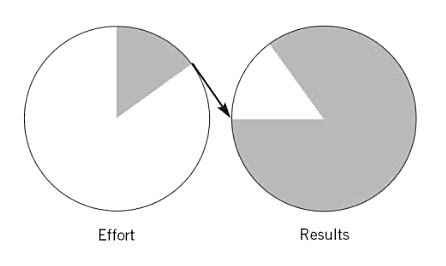
\includegraphics[width=\textwidth]{graphics/pareto-principle}

So, yeah. We're going to filter out the good stuff. You can take any given
field, throw out everything except the 100 best papers and textbooks, and they
probably wouldn't be much worse off -- and, hey, you'd avoid stuffing your head
with a lot of garbage that will end up being wrong in the future. So bonus.

\section{Skimming and Trashing}

So, how do you know what to throw out and what to keep? By skimming it, of
course. At this point, you're going to want to spend about 5 minutes with each
book and paper gathered, and discard those that don't seem promising.

Maybe there's a science to this. I don't know. It's not that hard. You look at a
book, you read the table of contents, maybe you check its Amazon reviews or
citation count. Then you make a decision: do I want to pursue this further?

If you can't see yourself digging more deeply into the book or paper in
question, there's no use keeping it. And if you're thinking something is maybe on
the fence, like it's readable, but going to be a slog, you're probably best off
pitching it.

I mean, not all of the time, like maybe its one of those papers that set the research
agenda for the next twenty years or sparked a new field. In those cases, you
should make an exception and read it anyways.

Plus, reading a bad paper is not that much of a time sink, anyways, at least not
usually. Bad books can take up about 10x more time, so I'd be even picker with
evaluating those.

\newthought{Remember, each resource} that you cut out of this stage of the
pipeline is one less thing that you're going to have to read through in the
future. It's like gaining an extra two hours of your life.\marginnote{``One of
  my most productive days was throwing away 1,000 lines of code.'' Ken Thompson}

So be ruthless. Be brutal. Salt the earth like Pope Boniface VIII salted Palestrina in 1299.\footnote{``I wanted to say like Rome salted Carthage, but that particular story turns out to be a 19th century invention. Who knew?''} Crush the papers with the vigor of Charles Martel at the Battle of Tours. Filter like natural selection! If
you spend an extra five minutes checking whether or not to pursue something
further, that's time well spent! You might gain a few hours in the future by
doing that.

Being thorough at this stage is totally worth it. Look up citation counts, read
reviews, check tables of content, flip through stuff -- is the math too advanced?
I repeat, for this and all things in life: \textit{You can probably just skip
  it.}

\section{Heuristics}

Yes, woo, okay. I hope you're pumped up. Now, let me give you some heuristics
for deciding what to throw out.

Easy books are often so worth it. A gentle introduction as the first few things
you read: keep these, these are a lifesaver.

Hard stuff tends to be overrated and, at the beginning, too hard to process
without additional expertise. It's harder to process, understand, and
remember, a triple penalty. You don't need it.

Oh, and remember: if at any stage you really need a book or paper again, it's a
download or a library checkout away. There's a very modest cost attached to
accidently pruning something, so not a big deal.

Another easy way to filter stuff: if it has a ton of citations, keep it. If it
doesn't have a ton of citations, but looks very relevant: keep
it. Super-specific, super-relevant papers to you often don't get attention from
larger audiences, but they can be great. Just one of those might solve
your problem.

If a paper is neither super relevant nor received more than 5 citations, get rid
of it. On the other hand, if a paper is not super relevant, but has received
more than 100 citations, you should probably read it, just so you can understand
what it is that other people are talking about. 

\newthought{Do research on} your research. Check things you can quantify: is it
super long? Maybe you don't need it, or you can just read a certain
chapter. Does it has poor Amazon reviews? You don't need it.

Check citations, Google for book reviews. Here's a tip (don't make this mistake):
parapsychology is not a science. It's for loons who want to be ``scientific'' about the supernatural, you know, ghosts and extrasensory powers and
stuff. Don't read any of that.

Popular books can sometimes be good, sometimes horrible. Not that useful of a heuristic. Check author credentials\footnote{Except for mine. Don't check mine.} -- although there are a lot of experts who
are terrible at exposition, so this is a noisy signal. 

\newthought{Keep meta-analyses.} Anything with a large sample size is going to be more useful
than anything with a smaller one. Here's a way to think about it: imagine that,
for every subject studied, you have to spend a minute considering the evidence.

So, for a paper on 400 subjects, that's six and a half hours. For one on 40,000,
that's about a month.

Yeah, sure, in real life you can read them at the same rate, but the amount of
evidence in the second one is two orders of magnitude larger, and should be
weighted as such.

Only you can prevent yourself from falling victim to scope insensitivity.

% tk maybe a larger section here about scope insensitivity

\section{A final pass}

Okay, let's say that you've done that. You've trimmed, cleaned, scrubbed, and pruned. I'd now do
a second pass. You're more familiar with what you've got. Check for resources that
share too much information with each other, that are more or less duplicates,
(two introductory textbooks?) and pick the best-seeming one.

The goal in this pass is to be more holistic about the whole thing. Try to see
where papers fit in with other papers, how the books connect into it. Try sorting by
date. Once you've done this and filtered out everything you can, you can move
onto the next step.

\section{Creating a reading list}

Now, you've got a whole bunch of papers, a couple of textbooks. You need to
organize it all into a reading list. Read this, then that, then this, and so on.

I once read 150 papers on happiness over the course of a summer. How? By reading
a couple of them each day, according to schedule. Less work than you might
think.

\newthought{But how?} How are you going to decide what to read when? First, remember that
when it's difficult to decide between two things, it's usually because they're
so similar that it's difficult to distinguish between the two.

\textbf{Fredkin's paradox:} many of the subjectively toughest decisions are the ones that
matter the most -- they're just so close that it's hard to tell them apart. 

With that heuristic in hand, what you want to do is create a system that fosters ``success spirals''. You want to facillitate in yourself a belief that you can do it (which
you totally can). The limiting factor in research journeys is not brainpower, but motivation and consistency.

Consistency is a separate topic. I'd have to write another book and I still
haven't figured it out, but you want to break it down into tasks that you're
going to do every day. I made it through my last big research session by
reading 60 book pages and at least 1 paper each day. You could do something similar.

As far as motivation goes, you don't want to come up against
papers that are too hard to read or too hard to understand, so save those for
when you have a better grasp of the field. In the beginning, focus on the
easiest and most relevant pieces of research.

And I mean \textit{easy}. If I wanted to go through a huge tour of statistics,
I'd probably start with something like \textit{The Cartoon Guide to
  Statistics}. Reading too hard or too dense books is a grueling affair, and you
need not do it unless absolutely necessary.

If at any point in the whole process, you're like, ``Man, this book sucks way
more than I thought'' just skip it. Alternatively, find a video you can
consume. Those are generally easier to understand, or maybe an audiobook -- whatever works. When I'm really delving into a topic, I
like to listen to podcasts about the topic when exercising or doing yardwork or whatever.

% tk probably audio and visual assets should be its own section + a section on
% listening at double the speed

Right, so, place the easy, broad introductions near the front of the list. After
or alongside those, place the review papers.

This is probably sufficient for now. Once you've exhausted those, you should
have a good idea of what to place next in the list, so come back then and replan
your next assault on the literature. (And, hey, if you did a good pruning job,
maybe you won't need to do anymore research.)

\section{Reading and Managing Information}

Someone once told me that their grad professor explained to them that their
duty as a student was like being a large walrus, and that you needed to swim
through the literature and hope that the important bits would get stuck to your
mustache.

I'd like to pause for a moment and, one, reflect on just what an awesome
metaphor that is and, two, how wrong it is. Like really wrong. Like Judas
killing Jesus level wrong. (But, okay, probably not \textit{that} wrong.)

The mind and memory
are not mysterious machines. You don't have to pray that they're going to
work.\marginnote{Why people say ``works like a charm'' shouldn't that mean that something, you know, \textit{doesn't work}?} You can find out (and you will find out when you get through the next chapters.)

So, yeah. You're going to swim through that literature, but you're not going to
hope. You're going to keep copious notes.

\section{Reading}

I'm going to paper over (heh) a lot of the difficulties and important parts
here, so that they can be more thoroughly covered in the other chapters.

But, basically, when reading all of this, there a few things you definitely,
seriously, absolutely need to do.

Reading a lot of stuff is mostly about setting some kind of daily page or time
quota, and just doing that. Each day. At 60 pages a day, you can absolutely plow
through books, but it can be a slog when it comes to dense prose.

You can instead do time budgets, but this is not as effective or motivating. If
you're into coffee, pair reading with coffee. If you're into meth, pair reading with meth.\footnote{The number of public intellectuals associated with more-than-casual amphetamine use is higher than you expect.}

\section{Highlighting}

Okay, I hope most of the material you collected is digital, because you're
going to want to be able to virtually highlight stuff and export it as
text. That way, you can search through it all later when you need to find
something. And, trust me, you're going to need to find something.

For this, I use the PDF reader Skim. It's simple, it works, it exports
highlights as text. That's all you need. When reading, just
highlight the important bits: anything you'd like to remember in the future.

\textit{Anything you don't record, you're going to forget.}

You should also keep a list of anything that you need to look into later. These are
often papers that you'd like to look up. Research is not a linear process. The
``collecting information'' stage continues during the ``doing research'' phase.

\section{Chapter Summaries}

When reading, your only duty is to pay attention and to highlight. You don't
need to do anything more than that. When you're done with a chapter, you should
write some sort of synthesis of that information. A brief chapter summary, maybe
with some bullets of the main bits.

These don't need to be as thorough as the highlights but naturally, the more
thorough you can make them, the better.

\section{Reviews}

When you've finished the book, you should read through your highlights
and incorporate those plus these chapter
summaries into something a bit larger: what the book is about, along with your
thoughts on the book.

Why are you going to go through all this pain? Because once you're finished
with reading all of the research and six months (or six years) down the road,
you're not even going to remember whether or not you've even read the book.

So, really, this is your only message you get to send to your future self, along
with your highlights, about the book. So I suggest you be pretty
thorough: write down what the book was about, what you learned, and what you
thought of it.

It's sometimes useful to imagine that you're writing this backwards in time, to
somebody smart, but who hasn't read the book. You know, like you, right now,
before you've begun.\marginnote{I think I got this tip from Feynman.}

So write down this long-form thing, maybe push it to a blog if you want,
whatever. Just do it.

Then, open up a file, in Word or emacs or wherever you write most of your text,
and write a brief paragraph about the book, along with its name. What you're
doing here, in essence, is creating your own annotated bibliography.

In the future, you're going to be asking, ``Wait, what was that book?'' and it's
going to be useful if you have one of these. I know. I should have made one, but
I didn't. These are absurdly valuable to yourself and to everyone who hasn't
slogged through the research, so do it. It's not that much work after reading a
book, either. Like 500 words, max.

That's the workflow for books.

\section{Yeah, but what about papers?}

With papers, you'll do the same thing, just on a smaller scale: write the
paragraph in your bibliography and do the highlights. That's probably
enough. For meatier or mind-blowing papers, do the final long-form writeup.

But no chapter summaries with papers. Those are sort of impossible and also
unnecessary.

\section{Evernote}

Finally, take all this stuff and upload it to Evernote or Google Docs. This way,
it's backed up, and you can easily search through it, which you're going to want
to know.

Because it's sort of useful to be able to say to someone (e.g. in an email)
``oh, there's a study on that,'' but it's much more impressive to say, ``Ah,
there's this study here, and they did this, but I thought this, this, and
this. Here are some excerpts.'' You know, a link, so that they can verify that you're not making it up
on the spot. Or mistaken. Lots of people are mistaken. About everything.

% tk add a section on the value of information

\section{Chapter review}

Congratulations, you've made it to the end of this chapter, and should
have a much better idea now about how to go about a serious research campaign.

But, as I'll reveal in the next chapter, you're almost certainly going to forget
90\% of everything you just read here within the next month (and maybe even the next 24 hours). 3 months or so down
the line, you may find yourself in a situation where you need a vetted research
workflow and, with luck, you'll recall reading this.

If you find your future self in such a scenario, just skip to this
section. Here's a summary of all the important parts of this chapter:

\begin{itemize}
\item The world is awash in information, so much that you can discover a new species
just by browsing Flickr. For any problem, there's some research that you should
be taking advantage of.

\item Research is much broader than libraries and laboratories. Googling a blind
date's name is research, as is reverse engineering your competitor's successes.

\item The single most important form of research is finding out the name of what it
is that you want to know. If you have the name of a spirit, you have power of
it.

\item For things you can't Google, like when you don't know the right words, you
must rely on human resources: your social network, experts, librarians, and Q\&A
sites, like Stack Exchange or Quora.

\item When it comes to learning about a field, use textbooks. That's what they're
custom tailored for.

\item Annotated bibliographies and recommended reading lists are extremely valuable
when it comes to amassing a bunch of relevant research.

\item Throwing out information is important. For each source you decide not to
investigate, you're saving hours or days of time. Thus, it makes sense to really
consider whether or not something is the worth reading -- is it the best source
of this information? Is reading it necessary?

\item Hard texts are overrated. They're emotionally and cognitively draining, hard to
understand, and hard to remember. Avoid them.

\item Structure reading of information from easy to hard. As you read, the once hard
texts will become easy, you'll have built up knowledge from the field, and will
get more out of the text.

\item When doing research, keep copious notes. Export highlights as text, write
chapter summaries, and write final book summaries. Assume that these documents
are all that future-you will retain in a year.

\item Remember: plain text is searchable. You can upload your notes to a platform
like Evernote or Google Docs and have it all at your fingertips.
\end{itemize}

\section{Further reading}

When it comes to finding information and research methods, I've only scratched
the surface -- well, okay, we went a little bit deeper than the surface. If you
Google ``how to do research'' you'll find a lot of blog posts that cover the
surface and nothing more.

But there's a lot more! Research librarians spend a significant chunk of their
lives finding information, and they've picked up a lot of specialized
knowledge about the inner workings of libraries, the sort of stuff that you and
me aren't privvy to (and, frankly, don't want to be.)

The single best guide to library research that I've read is the \textit{The
  Oxford Guide to Library Research} by Thomas Mann. It covers, in detail,
finding the right keywords and subjects, serendipity, along with some
information on topics I haven't mentioned, like searching through
microfilm. If you're looking for information that's not on the web, this is the
book.

After that, \textit{Looking for Information: A Survey of Research on Information
  Seeking} is the next step, although I must admit that I've only read bits and
pieces.

\newthought{If you're interested} in business related research, such as the
answers to questions like, ``How much money should I spend on research?'' check
out Douglas Hubbard's \textit{How to Measure Anything}.\marginnote{``If you don't
  know what to measure, measure anyways. You'll learn what to measure.''} The book covers how to
measure things that don't seem like they can be measured, a message I can
definitely get behind. If doing monte carlo simulations in Excel to calculate
risk excites you, check it out.

\newthought{Really, though,} the best way to improve your ability to find
information is to go looking for it. If an explanation isn't satisfying, go
deeper. When it comes to figuring things out, don't settle.

In the words of the great mathematician David Hilbert, ``[O]ur slogan shall be:
We must know — we will know!''

% TK Using Google Books search to focus in on an anecdote.
